\chapter{Literature Review}
 
%%%%%%%%%%%%%%%%%%%%%%%%%%%%%%%%%%%%%%%%%%%%%%%%%%%%%%%%%%%%
%%%%%%%%%%%%%%%%%%%%  NEW SECTION   %%%%%%%%%%%%%%%%%%%%%%%%
%%%%%%%%%%%%%%%%%%%%%%%%%%%%%%%%%%%%%%%%%%%%%%%%%%%%%%%%%%%%
\setcounter{equation}{0}

\section{System Description}

The system can be described based on the four phases: 
   \begin{enumerate}
        \item Obtaining input from images 
        \item Recognizing table structure from the answer script 
        \item Applying OCR on the obtained images
	\item Obtaining the required result as CSV files
    \end{enumerate}

\begin{figure}[h!]
    \centering
    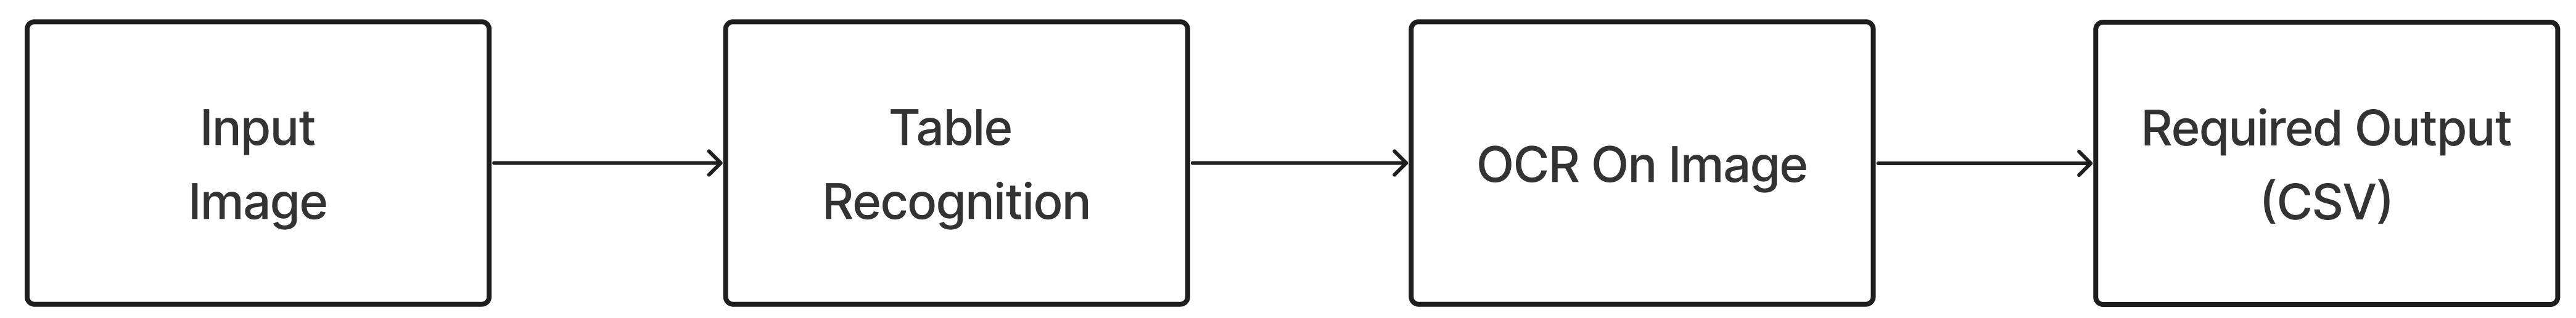
\includegraphics[width=1\textwidth]{Images/lit_review/Initial concept of our system.jpg}
    \caption{Initial concept of the system}
\end{figure}

\noindent The system uses a camera to accept images as input as per the requirements. This obtained input is then processed using the \textbf{img2table} library. Using this library, the table structure (i.e. cell coordinates) are extracted and cropped to obtain the values inside the cell. These values are then given to the TensorFlow OCR model to accurately classify and predict the values obtained from the cell extraction step. The obtained result from this step is arranged specially in the format of CSV files. 

\clearpage

\section{Existing Solutions}

\noindent
The system description was based on the initial concept that was pitched before extensive research. The phases of this system concept may have existing solutions of various implications and importance which will be explored below.\\

\noindent
Aaryan Raj et al. [1] proposed {\textit Revolutionizing Data Entry: An In-Depth Study of Optical Character Recognition Technology and Its Future Potential} in February 2023.
\noindent
It provides a comprehensive analysis of the history, current state, and future of OCR technology. By the concluding statements of this research journal, it was deduced that OCR technology is applicable for this system.\\

\noindent
Colin G. White-Dzuro et al. [7] proposed {\it Extracting Medical Information from Paper - COVID-19 Assessment Forms} in 2021. 
\noindent
It examines the validity of optical mark recognition, a novel user interface, and crowd-sourced data validation to rapidly digitize and extract data from paper COVID-19 assessment forms at a large medical center. Though this seems to be a good conclusion, the paper also warns that their proposed model is prone to errors and only guarantees an accuracy of 70\%.\\

\noindent
Jiayi Yuan et al. [8] proposed {\textit An OpenCV-based Framework for Table Information Extraction} in September 2020. 
\noindent
It proposes a novel OpenCV-based framework to extract the metadata and specific values from PDF tables. \\

\noindent
B.Gatos et al. [14] proposed {\textit Automatic Table Detection in Document Images} in 2005. 
\noindent
It proposes a workflow for table detection that comprises three distinct steps: (i) image pre-processing; (ii) horizontal and vertical line detection and (iii) table detection. The Probabilistic Hough Line Transform \textbf{(houghlinesp())} in the OpenCV package is discussed which can be used to create a bounding box around the desired cells that needed to be extracted. \\

\noindent This provided the system with a possible solution for table recognition and extraction. \\

\noindent
Abhishek Das et al. [9] proposed {\textit LSTM-based  Odia  Handwritten  Numeral Recognition} in September 2020.
\noindent
It focuses on the loss in recognizing the digits and is evaluated using the categorical cross-entropy loss function. The approach in focus here is LSTM\nomenclature{LSTM}{Long Short Term Memory}.\\

\noindent
Raajkumar G. et al. [11] proposed {\textit Optical Character Recognition using Deep Neural Network} in July 2020. 
\noindent
It aims at analyzing various text images like blurred and tilted images and it identifies the text from these images using deep learning models. The approach in focus here is CNN.\\

\noindent
The above two references provided possible options on what approach could be followed for the process of handwritten digit recognition.\\

\noindent
Chen ShanWei et al.[6] proposed {\textit A CNN-based Handwritten Numeral Recognition Model for Four Arithmetic Operations} in 2021. It proposes an automatic checking system based on CNN for handwritten numbers. By the concluding statements of this journal, it was confirmed that CNN must be the backbone of the proposed system. In future scope implementations, it is suggested to add layers of LSTM to compare the difference between the previous and updated versions of the model. \\

\noindent
Ömer Aydin [4] proposed {\textit Classification of Documents Extracted from Images with Optical Character Recognition Methods} in June 2021. 
\noindent
It focuses on the fact that handwriting or printed documents have been digitalized by a scanner or digital camera and these documents have been processed with two different OCR operations. \\

\noindent
Sachin Shrivastava et al. [5] proposed {\textit CNN-based Automated Vehicle Registration Number Plate Recognition System} in March 2021.
\noindent
It focuses on the different methods of VRNPR\nomenclature{VRNPR}{Vehicle Registration Number Plate Recognition} and emerging technologies that are used to get accurate results. \\

\noindent
These research papers helped gain more perspective and understanding of how CNN can be applied to real-life scenarios and situations of the most importance.

\clearpage

\noindent
Bjorn Barz et al. [12] proposed {\textit Deep Learning on Small Datasets without Pre-Training using Cosine Loss} in May 2020. 
\noindent
It shows that the cosine loss function provides substantially better performance than cross-entropy on datasets with only a handful of samples per class. \\

\noindent
According to the TensorFlow documentation, it is possible to apply the sparse categorical cross-entropy function. This is made possible because the labels for the number images stored in the folders have the same names as the folders themselves. \\

\noindent
Akkem Yaganteeswarudu [10] proposed {\textit Multi Disease Prediction Model by using Machine Learning and Flask API} in July 2020. 
\noindent
It focuses on Python pickling, which is used to save the model behavior, and Python unpickling, which is used to load the pickle file whenever required. Using the conclusion from this paper, Flask API stands out to be the better tool that can be used to create a simple yet appealing application interface.


\section{Summary}

\noindent 
The literature review presented a thorough examination of different research studies and works relevant to the proposed system. It offered valuable insights and multiple potential solutions for addressing each phase of the development of the system.

\vspace{3mm}

\noindent
Firstly, the comprehensive analysis of OCR technology [1] provided a very good understanding of the history, current state, and potential future advancements in this field. This analysis proved to be crucial in determining the most appropriate OCR technology to be integrated into the proposed system. By identifying the strengths and limitations of various OCR techniques, the study guided the selection of the most suitable technology to ensure accurate and efficient digit recognition from the answer script images.

\vspace{3mm}

\noindent
Moreover, the research overviews on table extraction [8] and table detection [14] methods contributed significantly to the development of the capability of the system to detect and extract table structures from the scanned answer scripts.

\clearpage

\noindent
By exploring different approaches and algorithms, these studies offered valuable insights into the most effective methods for identifying and capturing tabular data. Consequently, this enabled the system to accurately process and interpret table information, which is often an essential part of academic and assessment-related documents.

\vspace{3mm}

\noindent
Furthermore, the comparison study conducted in [9] and [11] was instrumental in determining the optimal approach for the implementation of the system. By evaluating LSTM and CNN models, the research highlighted the unique strengths of each method and their suitability for different aspects of the system. As a result, it provided the necessary knowledge for making informed decisions on how to leverage both LSTM and CNN effectively within the proposed system, ensuring enhanced performance and accuracy in various processing tasks.

\vspace{3mm}

\noindent
The discussions on the applications of CNN and LSTM in different contexts [4], [5], and [6] further corroborated the suitability of the chosen approaches for the proposed system. By analyzing how these models have been successfully deployed in diverse scenarios, the literature showcased the versatility and efficacy of CNN in handling image-related tasks and reinforced the decision to integrate it into the system.

\vspace{3mm}

\noindent
Lastly, the focus on Python pickling and unpickling methods [10] offered insights into an efficient means of serializing and deserializing Python objects. Drawing from this study, the suggestion to utilize Flask API for building the user interface of the proposed system emerged as a pragmatic approach. The lightweight and versatile nature of Flask API, along with the compatibility with the pickling methods in Python, made it an ideal candidate for providing a user-friendly interface to interact with the system. 

\vspace{3mm}

\noindent
According to this, each phase of the proposed system is planned, which will be discussed in the subsequent chapter.

